\chapter{Application : recherche de bugs dans Radare2}

Afin de mettre en application le fuzzing avec AFL, nous avons ciblé le logiciel Radare2 (logiciel libre disponible sur \href{https://github.com/radare/radare2}{github}) afin de découvrir de potentiels problèmes dans celui-ci.
Radare2 est un logiciel de reverse-engineering open-source et développé activement par une large communauté.
Il s'agit d'ailleurs d'une suite d'outils (radare2, rasm2, rax2, rafind2...) permettant entre autre de désassembler des binaires pour un nombre important d'architectures (x86, ARM, MIPS...), d'obtenir des informations sur de nombreux formats (ELF, PE, MACHO...), etc.

Nous avons décidé de cibler Radare2 étant donné qu'il possède une surface d'attaque assez importante et qu'il s'agit d'un logiciel de plus en plus utilisé dans le domaine du reverse-engineering.

\section{Méthodologie}

Notre approche concernant le fuzzing de Radare2 s'est déroulé comme suit :

\begin{itemize}
\item Récupération des sources et compilation de AFL ;
\item Récupération des sources de Radare2, et compilation de celui-ci avec \lstinline{afl-gcc} afin d'instrumenter le programme ;
\item Compréhension de la suite d'outils de Radare2, ciblage des entrées utilisateur et écriture des jeux des tests ;
\item Lancement de plusieurs instances d'AFL sur nos jeux de tests précédents ;
\item Analyse des crashs obtenus et des différentes mutations avec ASAN.
\end{itemize}

\subsection{Installation de AFL}

Pour récupérer les sources de AFL, il suffit de se rendre sur le site de Icamtuf (\href{http://lcamtuf.coredump.cx/afl/releases/afl-latest.tgz}{afl-latest}) pour récupérer l'archive, et de compiler le compiler en tapant simplement \lstinline{make} une fois décompressée.

\subsection{Instrumentation de Radare2 grâce à \lstinline{afl-gcc}}

Nous avons compilé deux versions de Radare2 : une version normale instrumentée avec \lstinline{afl-gcc} et une autre compilée avec ASAN afin de découvrir de nouveaux problèmes.
La première version peut se compiler de cette manière :

\begin{lstlisting}
  $ git clone https://github.com/radare/radare2.git radare2
  $ mkdir radare2-install
  $ cd radare2
  $ CC=path-to-afl-gcc ./sys/user.sh --install-path ../radare2-install
\end{lstlisting}

Pour obtenir une version compilée avec ASAN, nous pouvons utiliser ces commandes :

\begin{lstlisting}
  $ git clone https://github.com/radare/radare2.git radare2-asan
  $ mkdir radare2-install-asan
  $ cd radare2-asan
  $ CC=path-to-afl-gcc AFL_USE_ASAN=1 ./sys/user.sh --install-path ../radare2-install-asan
\end{lstlisting}

Il faut savoir que ASAN peut difficilement être utilisé avec AFL.
En effet, en moyenne, l'instrumentation effectuée par ASAN multiplie par 3.4 la mémoire utilisée par le programme\cite{asan}, et qu'alors AFL limite la quantité de mémoire utilisée pendant le fuzzing d'un programme pour préserver la stabilité du système.
Pour pouvoir l'utiliser avec AFL il aurait été nécessaire de le compiler en 32bits, ce que nous n'avons pas réussi à faire sur les serveurs du CREMI.

\subsection{Écriture des entrées initiales pour le fuzzing}

Maintenant, il est nécessaire de choisir quels sont les parties de Radare2 que nous souhaitons tester avec AFL.
Nous avons tenté de fuzzer les composants suivants :

\begin{itemize}
\item radare2 : il s'agit du programme principal du projet Radare2.
  Celui-ci peut prendre en paramètre des scripts exécutant des commandes et un fichier binaire à analyser.

  Nous avons choisi de tester à la fois le parsing des scripts passés à radare2, et à la fois le parser des formats de fichiers binaires.
\item rasm2 : il s'agit d'un programme permettant de désassembler des instructions codées en hexadécimal passées dans un fichier.
\item rax2 : une calculatrice supportant plusieurs bases (binaire, hexadécimal).
\item rafind2 : un outil permettant de donner des informations sur le type de fichier passé en paramètre (à la manière de la commande \lstinline{file}).
\item rabin2 : un outil pouvant donner différentes informations sur le fichier binaire passé en paramètre (sections, segments...).
\end{itemize}

Pour fuzzer les formats de fichiers, nous avons utilisé le dépôt \href{https://github.com/JonathanSalwan/binary-samples}{binary-samples} en utilisant les binaires les plus petits de chaque format afin d'accélérer le fuzzing.

Pour les outils \lstinline{rasm2}, \lstinline{rax2} et \lstinline{radare2} (partie scripts), nous avons simplement écrit un fichier valide minimal de quelques octets pour chaque outil.

\subsection{Lancement de \lstinline{afl-fuzz}}

Une fois tout ce travail effectué, nous avons lancé une instance de \lstinline{afl-fuzz} pour chaque partie du logiciel testé.
Pour cela, nous avons utilisé les serveurs de calculs (\path{mcgonagall.emi.u-bordeaux.fr}) mis à disposition du CREMI possédant pas moins de 48 CPUS AMD64 et 128 Go de mémoire RAM.
Après environ trois jours, nous avons obtenu un certains nombre de crashs grâce à nos jeux de tests et AFL.

Chaque instance de AFL peut être lancée de la manière suivante, où le dossier \path{in/} contient nos jeux de tests initiaux.
Par exemple, pour fuzzer les scripts de radare2 :

\begin{lstlisting}
  $ ./radare2/env.sh ./radare2-install
  $ afl-fuzz -i in -o out -m 256M ./radare2-install/bin/radare2 -i @@ -q /sbin/ebtables
\end{lstlisting}

Ici, les caractères '@@' seront remplacés par le fichier muté par AFL, c'est à dire le script initial du dossier \path{in/} avec les modifications appliquées par \lstinline{afl-fuzz}.

Ci-dessous, le résultat d'une des instances de AFL lancée sur l'outil \lstinline{radare2} :

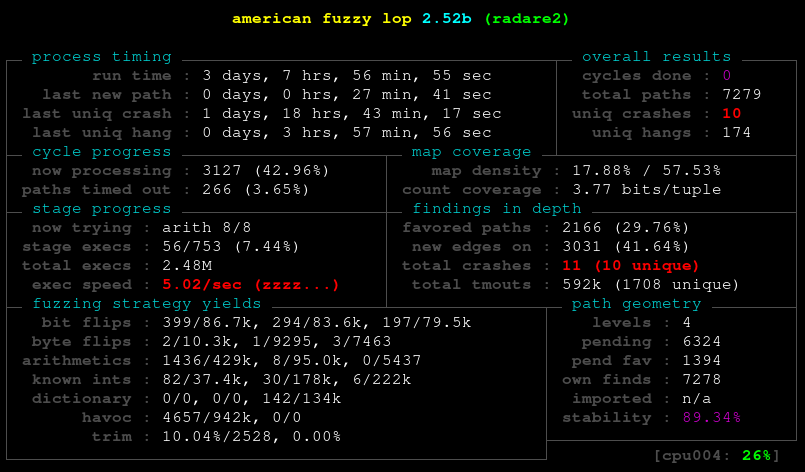
\includegraphics[width=0.9\linewidth]{../medias/afl-fuzz.png}

\subsection{Analyse des résultats obtenus}

Après quelques jours de fuzzing, nous avons obtenus dix crashs sur le parsing des commandes \lstinline{radare2} et un crash sur le parsing des fichiers binaires (toujours sur l'outil \lstinline{radare2}).
Les fichiers générant ces crashs sont stockés dans le dossier \path{out/crashes/}, les entrées s'exécutant en plus d'une seconde (temps de timeout par défaut de AFL) dans le dossier \path{out/hangs/} et l'ensemble des mutations dans le dossier \path{out/queue/}.

Afin de découvrir d'autres problèmes potentiels, nous avons réexécuté notre version de Radare2 compilée avec ASAN sur l'ensemble des fichiers présents dans \path{out/queue/}.
Cela nous a permis de découvrir notamment un problème dans l'outil \lstinline{rax2} et d'autres problèmes dans le parsing des scripts de \lstinline{radare2}.
L'analyse de ces différents problèmes sont présentés dans la section suivante.

\section{Problèmes constatés}
